\documentclass[String-lecture-21.tex]{subfiles}

\begin{document}
\section{Type II superstring theories}\label{sec:TypeII}
We have seen that the triality $\bf 8_v$, $\bf 8_s$, $\bf 8_c$ of the eight-dimensional irreducible representations of $\SO(8)$ appear as the massless spectrum of the RNS superstring theory after the GSO projections. One way to explain the critical dimension $D=10$ of superstring theory is that the little group $\SO(8)$ of the Lorentz group $\SO(1,9)$ of the spacetime has these special eight-dimensional irreducible representations. As explained, the GSO projections \eqref{GSO-R} in the R sector pick one of the irreducible spinor representations $\bf 8_s$, $\bf 8_c$ of $\SO(8)$. In this section, we will obtain superstring theories of two different types, depending on the sign in the GSO projection operators. The analysis of massless fields in Type II theories predicts extended objects, called \textbf{D-branes} \cite{Polchinski:1995mt}.

\subsection{Type II superstrings}\label{sec:Type2}
Like bosonic closed string theory, massless spectrum even in closed superstring can be determined by taking tensor products of massless states in the left- and right-moving sector. However, we now have a choice between  $\bf 8_s$ and $\bf 8_c$ in the R sector. Hence, there are two inequivalent ways to construct superstring theory: the same (IIB) or opposite (IIA) choices on the right- and left-moving spectrum.
These lead to the massless sectors
\begin{align}\label{IIA-IIB}
{\rm Type ~ IIA\colon} & ({\bf 8_v}\oplus{\bf 8_s}) \otimes
   ({\bf 8_v}\oplus{\bf 8_{c}}) \nonumber\\
{\rm Type ~ IIB\colon} & ({\bf 8_v}\oplus{\bf 8_s}) \otimes
   ({\bf 8_v}\oplus{\bf 8_{s}})
\end{align}
of $\SO(8)$. Although one can also choose
\begin{align}
{\rm Type ~ IIA'\colon} & ({\bf 8_v}\oplus{\bf 8_c}) \otimes
   ({\bf 8_v}\oplus{\bf 8_{s}}) \nonumber\\
{\rm Type ~ IIB'\colon} & ({\bf 8_v}\oplus{\bf 8_c}) \otimes
   ({\bf 8_v}\oplus{\bf 8_{c}})
\end{align}
they are equivalent after the spacetime parity redefinition. By the construction, Type IIB theory is chiral whereas IIA theory is not chiral. Also, the tensor products of the NS-NS and R-R sectors provide massless bosonic fields whereas those of the NS-R and R-NS sectors give massless fermionic fields.

\begin{table}[ht] \centering
\begin{tabular}{ |c|c|c| }
 \hline
 IIA & ${\bf 8_v}$ & ${\bf 8_c}$ \\ \hline
 ${\bf 8_v}$ & ${\bf 1} \oplus {\bf 28}  \oplus {\bf 35}$ & ${\bf 8_s}\oplus{\bf 56_c}$ \\
  & $\phi \ \ B_{\mu\nu} \ \ G_{\mu\nu}$ & $\lambda^+ \ \ \psi^-_m$ \\ \hline
  ${\bf 8_s}$ & ${\bf 8_c}\oplus{\bf 56_s}$ & ${\bf 8_v} \oplus
{\bf 56_t}$ \\
    & $\lambda^- \ \ \psi^+_m$ & $C_n \ \ C_{nmp}$ \\
 \hline
\end{tabular}
\hspace{2cm}
\begin{tabular}{ |c|c|c| }
 \hline
 IIB & ${\bf 8_v}$ & ${\bf 8_s}$ \\ \hline
 ${\bf 8_v}$ & ${\bf 1} \oplus {\bf 28}  \oplus {\bf 35}$ & ${\bf 8_c}\oplus{\bf 56_s} $ \\
  & $\phi \ \ B_{\mu\nu} \ \ G_{\mu\nu}$ & $\lambda^+ \ \ \psi^-_m$  \\ \hline
  ${\bf 8_s}$ & ${\bf 8_c}\oplus{\bf 56_s} $ & ${\bf 1} \oplus {\bf 28}  \oplus {\bf 35}_+$ \\
    & $\lambda^+ \ \ \psi^-_m$  & $C \ \ C_{mn}\ \ C_{mnpq}$ \\
 \hline
\end{tabular}
\caption{Massless fields in Type IIA and IIB theory.}\label{tab:masslessII}
\end{table}


Let us first look at the massless bosonic sector.    In the NS-NS sector, this is the same as bosonic string theory
\be
{\bf 8_v} \otimes {\bf 8_v} = \phi \oplus B_{\mu\nu} \oplus G_{\mu\nu}
={\bf 1} \oplus {\bf 28}  \oplus {\bf 35} .
\ee
Thus, the new ingredients come from the R-R sector, and the IIA and IIB spectra are respectively
\begin{align}
{\bf 8_s} \otimes {\bf 8_c} &= [1] \oplus [3] = {\bf 8_v} \oplus
{\bf 56_t} \nonumber\\
{\bf 8_s} \otimes {\bf 8_s} &= [0] \oplus [2] \oplus [4]_+
= {\bf 1} \oplus {\bf 28}  \oplus {\bf 35}_+ ~.
\end{align}
Here $[n]$ denotes the $n$-the antisymmetric representation of
$\SO(8)$, and we associate R-R $n$-form $C_{(n)}$ to it.
Also, here  $[4]_+$ means its R-R field strength $G_{(5)}=dC_{(4)}$ is self-dual
\be\label{SD-5form} \ast G_{(5)}=G_{(5)}~.\ee
 Note that the representations
$[n]$ and $[8-n]$ are related by the Hodge dual so that they are related by contraction with the
8-dimensional $\epsilon$-tensor. As we will see next, these R-R fields are associated to D-branes in Type II theories, and $[n]$ and $[8-n]$ are related by the electro-magnetic duality.


Let us first look at the massless fermionic sector.
The tensor products of the NS-R and R-NS sectors are given by
\begin{align}
{\bf 8_v} \otimes {\bf 8_c} &=
{\bf 8_s}\oplus{\bf 56_c} \nonumber\\
{\bf 8_v} \otimes {\bf 8_s} &=
{\bf 8_c}\oplus{\bf 56_s}~.
\end{align}
The $\bf 56_{s,c}$ correspond to gravitinos $\psi^\pm_{m,\a}$ that are superpartners of gravitons, and they have vector and one spinor indices by construction. As we will see in \S\ref{sec:supergravity}, they will give spacetime supersymmetry.  The $\bf 8_{s,c}$ are dilatino $\lambda^\pm_{\a}$ which are superpartners of the dilaton field.


\subsection{Introduction to D-branes}\label{sec:intro-Dbrane}


The massless spectrum from closed strings analyzed above does not incorporate gauge fields because gauge fields arise from an open string.
To incorporate open strings in Type II theories, we need to introduce D-branes.
Note that closed superstring theories are consistent in themselves as we see in Heterotic string theory \S\ref{sec:Heterotic}.
However, only open string theory is inconsistent,
and it requires closed strings as well (see Figure \ref{OpenClosed}).
\begin{figure}[htb]
\centerline{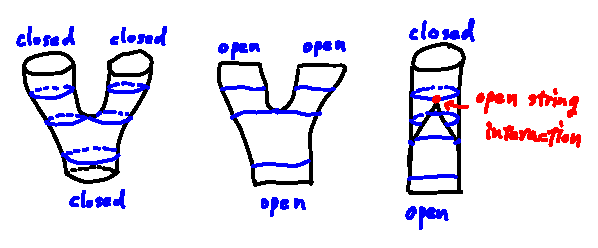
\includegraphics[width=350pt]{picture/OpenClosed}}
\caption{Open string interaction induces closed string}
\label{OpenClosed}
\end{figure}

\subsubsection*{Boundary conditions \& D-brane}

As seen in \eqref{open-variation}, we have imposed the two types of boundary conditions for open strings.
In fact, the Dirichlet boundary condition (Figure \ref{BoundaryObj}) does not conserve the momenta of open strings (exercise).
It implies that there must be an object into which the momentum goes.
We call this object a D-brane where the D stands for Dirichlet and
brane comes from the membrane. Indeed, we can impose the Neumann boundary condition to some coordinates and the Dirichlet to the other coordinates:
\begin{align*}
 &\textrm{Neumann condition on } X^a \quad (a=0,1,\ldots,p)  \\
 &\textrm{Dirichlet condition on } X^I \quad (I=p+1,\ldots,D-1)
\end{align*}
The corresponding D-brane is called a \textbf{D$p$-brane}, which extends to a $p$-dimensional subspace or a $(p+1)$-dimensional spacetime.
Now we can visualize a configuration of D-brane and string as in Figure \ref{BoundaryObj}.
A D-brane is a dynamical object as it should receive the momentum so that it has action and interactions with string. (See \S\ref{sec:D-brane}.)
On the other hand, in order to give the Dirichlet boundary condition $X^I = c^I$,
a D-brane must be infinitely heavier than a string.



\begin{figure}[ht]\centering
\raisebox{1cm}{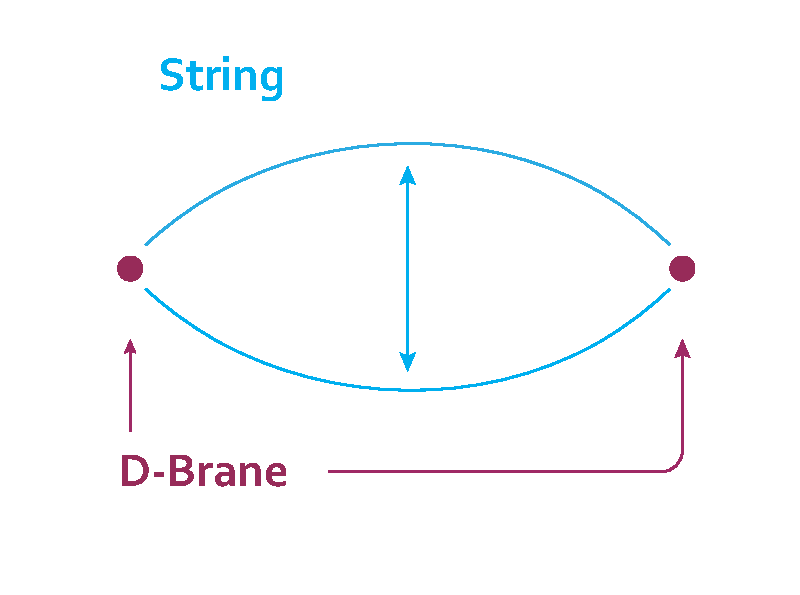
\includegraphics[width=6cm]{picture/BoundaryObj}}\hspace{1cm} \includegraphics[width=8cm]{picture/DpBrane}
\caption{D-brane must exist at the ends of the open string so that momentum can escape from the string.}
\label{BoundaryObj}
\end{figure}




\subsubsection*{Chan-Paton factor}

We can consider not only a single D-brane but also a stack of D-branes,
and a string now has a choice of D-branes to which a string ends.
Let us label this option $i$ ($i=1,\ldots,n$), which is called \textbf{Chan-Paton factor}.
As an open string has two endpoints, Chan-Paton degree of freedom is specified by
\begin{align}\label{CP-factors}
 |N;k \rangle  \quad  \to \quad |N;k;ij \rangle \ .
\end{align}
Now we have $n^2$ massless vector states in both bosonic string and superstring theory.
As usual, we use $n \times n$ Hermitian matrices $T^a$ normalized to
\begin{align*}
 \Tr (T^a T^b) = \delta^{ab} \ ,
\end{align*}
which consist of a complete set for data of the open string endpoints:
\begin{align}\label{CP-factor2}
 |N=1;k;a \rangle = T^a_{ij} |N=1;k;ij \rangle \ .
\end{align}
These states correspond to a $\U(n)$ gauge field. (You can check it by a three-point amplitude.)



Note that in order to realize $\U(n)$ gauge group, the D-branes must coincide at a point.
Otherwise, the gauge group is broken by Higgs mechanism (see Figure \ref{ManyD}).
\begin{figure}[htb]
\centerline{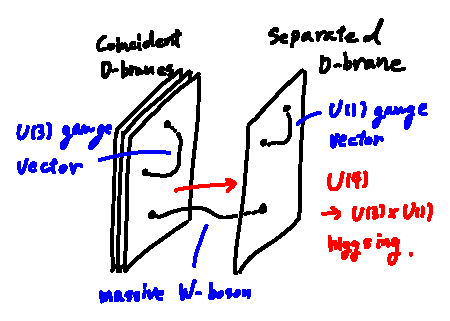
\includegraphics[width=13cm]{picture/ManyD}}
\caption{Many D-branes and Chan-Paton factors. $\U(n)$ gauge group and Higgs mechanism.}
\label{ManyD}
\end{figure}


We will see in \S\ref{sec:orientifold} that other types of gauge groups ($\SO$ or $\Sp$) can be realized in string theory with orientifold planes.



\subsubsection*{D-brane in IIA/IIB superstring theory}

D-branes arise as boundary conditions of open strings, and they carry gauge fields. Since D-branes are intrinsic to string theory, it reveals many interesting facets so that we will further investigate their properties.
In \S\ref{sec:Type2}, we saw that Type II superstring theories are endowed with R-R fields,
which are anti-symmetric tensors analogous to gauge fields.
Like an electron/monopole is coupled to the gauge fields,
D-branes are coupled to the R-R fields in Type II theories.


To use the analogy of electromagnetism, let us quickly review an electron/monopole interacting with the electromagnetic fields in the $(3+1)$-dim spacetime.
An electron is expressed by a source
\[J^\mu = (\rho, \bfj) = (q \delta^3(\bfr-\bfr(t)), \partial_t \bfr(t) \rho )~,\]
and its coupling to the gauge field $A$ is given by
\begin{align*}
 S_J = q_e \int A_\mu J^\mu d^4x = q_e \int_\gamma A_\mu dx^\mu = q_e \int_\gamma A \ ,
\end{align*}
where $q_e$ is an electric charge, and $\gamma$ is the world-line of the electron. Since the Maxwell equation is \be\label{Maxwell}\ast d \ast F_{(2)}= J_e\ee, we can obtain the electric charge by
\[
q_e=\int_{S^{2}} \ast F_{(2)}~.
\]
On the other hand, the electromagnetic duality
\be\label{Maxwell2}
 d  F_{(2)}= J_m\ee tells us that
a magnetic monopole is a source $J_m= q_m \delta^3(r)$ of a magnetic flux.
Therefore, the magnetic charge can be measured as
\begin{align*}
 q_m= \int_{S} F_{(2)} = \int_{B} d F_{(2)} \ ,
\end{align*}
where a surface $S$ around the monopole.
% the monopole, $B_3$ is a 3-dim ball, whose boundary is $S$,
% $B$ in the second line is $B_3$, and $\partial B$ is a surface of $B$, which is $S$.
% Note that $F_{(2)}$ cannot be expressed by an exterior derivative $dA$ globally,
% hence, $dF_{(2)} \neq 0$, rather $dF_{(2)} = \nabla \cdot B = q_m \delta^3(r)$.
It is well-known that the charges of the electron and monopole obey the Dirac quantization condition (for instance, see \cite[\S13.3]{Polchinski}):
\be
q_e q_m\in 2\pi \bZ~.
\ee



\begin{figure}[htb]
\centerline{\includegraphics[width=15cm]{picture/mono}}
\caption{Higher dimensional analog of monopole: magnetic flux of D$(6-p)$-brane.}
\label{mono}
\end{figure}


In a similar fashion, a D$p$-brane ($p\le 3$) supported on a world-membrane $M_{p+1}$  is electrically coupled to the R-R $(p+1)$-form $C_{(p+1)}$ as
\begin{equation}\label{RR-coupling}
 S_{p} = \mu_{p}\int_{M_{p+1}} C_{(p+1)} \ .
\end{equation}
where $\mu_{p}$ is the charge of the D$p$-brane.
An exterior derivative of the R-R potential
gives its R-R field strength $G_{(p+2)} = d C_{(p+1)}$, and its electromagnetic dual is given by its Hodge dual
\[
\widetilde{G}_{(8-p)}=\ast G_{(p+2)}
\]
From Gauss's law, the charge is given by the flux of $\widetilde{G}_{(8-p)}$ over a sphere $S^{8-p}$ around the D$p$-brane
\[
\mu_{p}=2\kappa_{10}^2\int_{S^{8-p}} \widetilde{G}_{(8-p)}~,
\]
where $2\kappa_{10}^{2}=(2 \pi)^{7} \alpha^{\prime 4}$.
The magnetic dual of the D$p$-brane is a D$(6-p)$-brane, and its magnetic charge is accordingly given by
\[
\mu_{6-p}=2\kappa_{10}^2\int_{S^{p+2}} G_{(p+2)}~.
\]
They must obey the Dirac quantization condition
\be\label{Dirac-quantization}
2\kappa_{10}^2\mu_{p}\mu_{6-p}\in 2\pi \bZ~.
\ee
Writing the flux $\wt G_{(8-p)}=d\wt C_{(7-p)}$, the D$(6-p)$-brane is magnetically coupled to  $\wt C_{(7-p)}$.
Now, reading off R-R fields from Table \ref{tab:masslessII}, we see that there are D$p$-branes for even $p$ in Type IIA and for odd $p$ in Type IIB theory.


\begin{figure}[htb]
\centerline{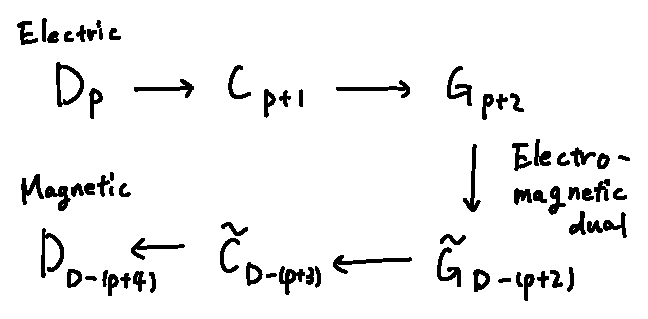
\includegraphics[width=10cm]{picture/EleMagD}}
\caption{Electro-magnetic duality and D-brane.}
\label{EleMagD}
\end{figure}

% If you allow to use electro-magnetic duality, it is more easily understood (see Figure \ref{EleMagD}).

Even from the NS-NS sector, we can predict the presence of an extended object in string theory.
A string or a fundamental string, denoted as F$1$, is electrically coupled to the $B$-field.
On the other hand, there is an object magnetically coupled to the $B$-field,
which is called \textbf{NS$5$-brane}. There are always fundamental strings and NS5-branes in string theory of five types.


In conclusion, we summarize extended objects in Type II superstring theory in Table~\ref{table:branetypeII}.
\begin{table}[htbp]
 \centering{
  \label{table:branetypeII}
\begin{tabular}{l|ccc}
  IIA & $B_{(2)}$ & $C_{(1)}$ & $C_{(3)}$ \\
\hline
  Electric & F$1$ & D$0$ & D$2$ \\
  Magnetic & NS$5$ & D$6$ & D$4$ \\
\end{tabular} \hspace{12pt}
\begin{tabular}{l|cccc}
  IIB & $B_{(2)}$ & $C_{(0)}$ & $C_{(2)}$ & $C_{(4)}^+$ \\
\hline
  Electric & F$1$ & D$(-1)$ & D$1$ & D$3$ \\
  Magnetic & NS$5$ & D$7$ & D$5$ & D$3$ \\
\end{tabular}
}  \caption{Extended objects in Type II superstring theory}
\end{table}
\vspace{2pt}

Note that a D$(-1)$-brane is a timely localized object (called an instanton). There are D$8$-branes in Type IIA theory, which are non-dynamical
so that there is no corresponding R-R anti-symmetric tensor. Moreover, these branes can be understood as a decay of the space-filling D9-brane and anti-D9-brane pair D9-$\overline{\textrm D9}$ \cite{Sen:1998tt}, which admits a beautiful mathematical interpretation \cite{Witten:1998cd} by K-theory.


\end{document}
